\documentclass{article}

\usepackage{listings}
\usepackage{hyperref}
\usepackage{todonotes}
\usepackage{verbatim}
\usepackage{tikz}
\usepackage{tkz-graph}
\usepackage{pgf}
\usetikzlibrary{arrows,automata}

% \newcommand*\beautier{\verb;beautier;}

\title{beautier: BEAUti for R}
\author{Rich\`el J.C. Bilderbeek}


% \newcommand*\filename[1]{${#1}$}
% \newcommand*\myfilename[1]{\verb;{#1};}

% Style of code
% From http://r.789695.n4.nabble.com/How-to-nicely-display-R-code-with-the-LaTeX-package-listings-tp4648110.html
\usepackage{fancyvrb} 
\definecolor{codegreen}{rgb}{0,0.6,0}
\definecolor{codegray}{rgb}{0.5,0.5,0.5}
\definecolor{codepurple}{rgb}{0.58,0,0.82}
\definecolor{backcolour}{rgb}{0.95,0.95,0.92}
\lstdefinestyle{mystyle}{
  language=R,% set programming language
  basicstyle=\ttfamily\small,% basic font style
  commentstyle=\color{gray},% comment style
  numbers=left,% display line numbers on the left side
  numberstyle=\scriptsize,% use small line numbers
  numbersep=10pt,% space between line numbers and code
  tabsize=2,% sizes of tabs
  showstringspaces=false,% do not replace spaces in strings by a certain character
  captionpos=b,% positioning of the caption below
  breaklines=true,% automatic line breaking
  escapeinside={(*}{*)},% escaping to LaTeX
  fancyvrb=true,% verbatim code is typset by listings
  extendedchars=false,% prohibit extended chars (chars of codes 128--255)
  literate={"}{{\texttt{"}}}1{<-}{{$\bm\leftarrow$}}1{<<-}{{$\bm\twoheadleftarrow$}}1
  {~}{{$\bm\sim$}}1{<=}{{$\bm\le$}}1{>=}{{$\bm\ge$}}1{!=}{{$\bm\neq$}}1{^}{{$^{\bm\wedge}$}}1,% item to replace, text, length of chars
  alsoletter={.<-},% becomes a letter
  alsoother={$},% becomes other
  otherkeywords={!=, ~, $, \&, \%/\%, \%*\%, \%\%, <-, <<-, /},% other keywords
  deletekeywords={c}% remove keywords 
}
\lstset{style=mystyle}

\begin{document}

\maketitle

\begin{abstract}
  \textbf{1. }
  Here, I present a package, \verb;beautier;, 'BEAUti for R', for the R programming language. \\
  \textbf{2. }
    \verb;beautier; allows for scripted use of the BEAST2 phylogenetics tool, 
    by creating BEAST2 input files from an R function call. \\
  \textbf{3. }
    I describe \verb;beautier; usage, the novel functionality it provides
    compared to BEAUti, and give some minimal examples. \\
  \textbf{4. }
    As \verb;beautier; is free, libre, open-source and designed to be extended, 
    I conclude by describing the current development of the package \\
\end{abstract}

% Key-words: computational biology, evolution, phylogeny, BEAST2, R

%%%%%%%%%%%%%%%%%%%%%%%%%%%%%%%%%%%%%%%%%%%%%%%%%%%%%%%%%%%%%%%%%%%%%%%%%%%%%%%%%%%%%%
\section{Introduction}
%%%%%%%%%%%%%%%%%%%%%%%%%%%%%%%%%%%%%%%%%%%%%%%%%%%%%%%%%%%%%%%%%%%%%%%%%%%%%%%%%%%%%%

BEAST2 \cite{bouckaert2014beast} is a popular Bayesian phylogenetics tool.
BEAST2 is bundled with the program called BEAUti \cite{drummond2012bayesian}.
BEAUti has a user-friendly graphical user interface to create BEAST2 input files,
but does not allow for the scripted use of BEAST2. '
\verb;beautier; does allow for scripted use of BEAST2 from an R function call.
An additional novelty is that \verb;beautier; allows to specify a fixed crown age.

%\begin{figure}
%  \centering
%  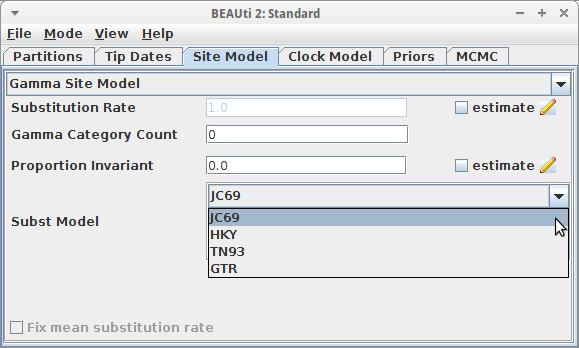
\includegraphics[]{BeautiSiteModel.png}
%  \caption{BEAUti}
%  \label{figure:beauti}
%\end{figure}


%%%%%%%%%%%%%%%%%%%%%%%%%%%%%%%%%%%%%%%%%%%%%%%%%%%%%%%%%%%%%%%%%%%%%%%%%%%%%%%%
\begin{figure}
  \centering
  \begin{tikzpicture}[->,>=stealth',shorten >=1pt,auto,node distance=6cm, semithick]   
  \tikzstyle{every state}=[]
  \node[state] (A) [rectangle] {
    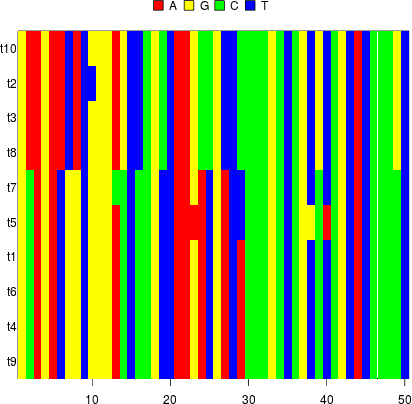
\includegraphics[width=0.2\textwidth]{alignment.png}
    
\includegraphics[width=0.2\textwidth]{thought_cloud.png}
  };   
  \node[state] (E) [below of=A, rectangle] {
    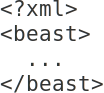
\includegraphics[height=0.1\textheight]{xml.png}
  };   
  \node[state] (F) [rectangle, below of=E] {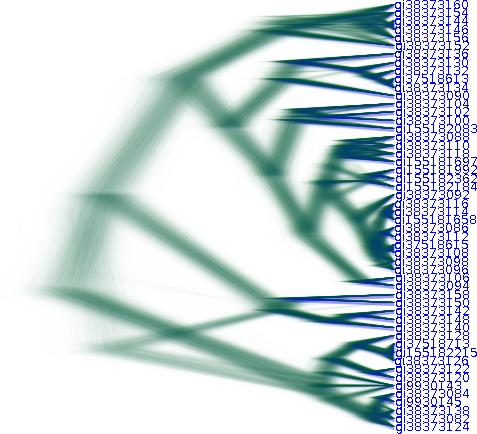
\includegraphics[width=0.3\textwidth]{DensiTreeExample2.jpg}};
  \path (A) edge [anchor = east] node {
\includegraphics[height=0.15\textheight]{beautier_logo.png}} (E)
        (A) edge [anchor = west] node {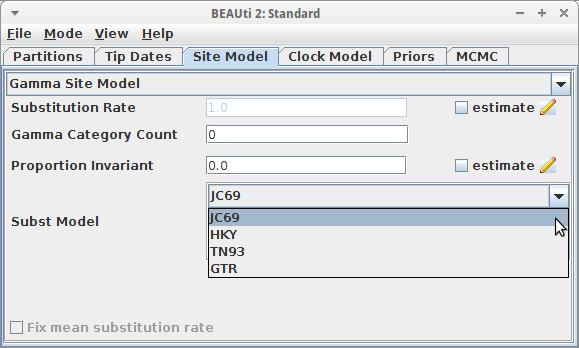
\includegraphics[height=0.15\textheight]{BeautiSiteModel.png}} (E)
        (E) edge [] node {
\includegraphics[width=0.2\textwidth]{Beast2LogoRat.png}} (F); 
  \end{tikzpicture}

  \caption{
    Workflow. From an alignment and priors, one creates a BEAST2 XML input file. This
    can be done using beastscript and BEAUti. The XML file created is run by BEAST2
    to create a posterior.
  }
  \label{fig:workflow}
\end{figure}
%%%%%%%%%%%%%%%%%%%%%%%%%%%%%%%%%%%%%%%%%%%%%%%%%%%%%%%%%%%%%%%%%%%%%%%%%%%%%%%%

%%%%%%%%%%%%%%%%%%%%%%%%%%%%%%%%%%%%%%%%%%%%%%%%%%%%%%%%%%%%%%%%%%%%%%%%%%%%%%%%%%%%%%
\section{Descriptions}
%%%%%%%%%%%%%%%%%%%%%%%%%%%%%%%%%%%%%%%%%%%%%%%%%%%%%%%%%%%%%%%%%%%%%%%%%%%%%%%%%%%%%%

\verb;beautier; is written in the R programming language \cite{R}.
\verb;beautier; creates the BEAST2 input files from an R function call.

\verb;beautier;'s main function is \verb;create_beast2_input_file;, which creates
an BEAST2 input file. 

\verb;create_beast2_input_file; needs at least the name of a FASTA file containing a DNA alignment
and a name for the to-be-created output file. This interface follows BEAUti's default settings.
Per alignment, a site model, clock model and tree priors can be chosen.
Multiple alignments can be used, each with its own (unlinked) site model, clock model and tree prior.


\begin{table}[]
\centering
\begin{tabular}{ | l | l | }
\hline
\textbf{Name} & \textbf{Description} \\
\hline
\verb;create_beast2_input_file; & Creates a BEAST2 input file \\
\hline
\verb;create_gamma_site_model; & Create a gamma site model \\
\verb;create_gtr_site_model; & Create a GTR site model \\
\verb;create_hky_site_model; & Create an HKY site model \\
\verb;create_jc69_site_model; & Create a Jukes-Cantor site model \cite{cantor1969mammalian} \\
\verb;create_tn93_site_model; & Create a TN93 site model \\
\hline
\verb;create_rln_clock_model; & Create a relaxed log-normal clock model \\
\verb;create_strict_clock_model; & Create a strict clock model \\
\hline
\verb;create_bd_tree_prior; & Create a birth-death tree prior \cite{kendall1948generalized} \\
\verb;create_cbs_tree_prior; & Create a coalescent Bayesian skyline tree prior \\
\verb;create_ccp_tree_prior; & Create a coalescent constant-population tree prior \\
\verb;create_cep_tree_prior; & Create a coalescent exponential-population tree prior \\
\verb;create_yule_tree_prior; & Create a Yule tree prior \cite{yule} \\
\hline
\verb;create_beta_distr; & Create a beta distribution \\
\verb;create_exp_distr; & Create an exponential distribution \\
\verb;create_gamma_distr; & Create a gamma distribution \\
\verb;create_inv_gamma_distr; & Create an inverse gamma distribution \\
\verb;create_laplace_distr; & Create a Laplace distribution \\
\verb;create_log_normal_distr; & Create a log-normal distribution \\
\verb;create_normal_distr; & Create a normal distribution \\
\verb;create_one_div_x_distr; & Create a 1/X distribution \\
\verb;create_poisson_distr; & Create a Poisson distribution \\
\verb;create_uniform_distr; & Create a uniform distribution \\
\hline
\end{tabular}
\caption{beautier's functions}
\label{tab:functions}
\end{table}

In total, \verb;beautier; has more than 150 exported functions to create
any    
By creating BEAST2 input files in BEAUti, 
the desired output of \verb;beautier; was determined. 
The functionality of BEAUti is added gradually (and is still growing).

\verb;beautier; has only parts of the functionality of BEAUti, yet
can be extended easily. \verb;beautier;, on the other hand, does allow for specifying
to use phylogenies of fixed crown age.

\verb;beautier; has a novel functionality not built into BEAUti yet:
it allows for using phylogenies of a fixed crown age. 

\verb;beautier; does not support the full functionality of BEAUti. Considering
the size, age and number of plugins, this would be close to impossible.
To compensate for this, an extensible software architecture is used.

\verb;beautier; has minimal support for calling BEAST2 from within R and does
so for testing purposes only. 

\verb;beautier; has minimal support for parsing and interpreting BEAST2 output files,
for that the \verb;RBeast; \cite{RBeast} package is recommended.

%%%%%%%%%%%%%%%%%%%%%%%%%%%%%%%%%%%%%%%%%%%%%%%%%%%%%%%%%%%%%%%%%%%%%%%%%%%%%%%%%%%%%%
\section{Examples}
%%%%%%%%%%%%%%%%%%%%%%%%%%%%%%%%%%%%%%%%%%%%%%%%%%%%%%%%%%%%%%%%%%%%%%%%%%%%%%%%%%%%%%

In R, a package's function need to be loaded in the global namespace first:

\begin{lstlisting}[language=R, caption=Loading, label=lst:loading_beautier, floatplacement=H]
library(beautier)
\end{lstlisting}

BEAUti, and likewise \verb;beautier;, need at least a FASTA filename
and an XML output filename. In BEAUti, this is achieved by loading a FASTA file (resulting
in figure \ref{fig:simplest_beauti_usage}), then saving an output file using a common
save file dialog. In \verb;beautier;, the same is achieved by listing \ref{lst:simplest_example}:

\begin{lstlisting}[language=R, caption=Simplest example, label=lst:simplest_example, floatplacement=H]
library(beautier)
create_beast2_input_file(
  "alignment.fas",
  "beast2.xml"
)
\end{lstlisting}

\begin{figure}
  \centering
  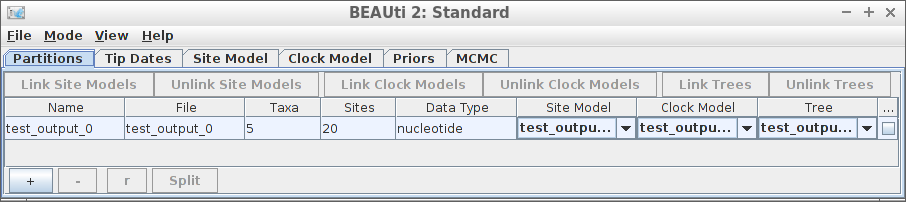
\includegraphics[width=\textwidth]{all_default.png}
  \caption{Simplest BEAUti usage}
  \label{fig:simplest_beauti_usage}
\end{figure}

This code will create a BEAST2 file with name '\verb;beast2.xml;',
using a FASTA file with name \verb;alignment.fas;, using the same default settings as BEAUti.
The default settings are, among others, to use a Jukes-Cantor site model \cite{cantor1969mammalian}, 
a strict clock, and a Yule birth tree prior \cite{yule}. Listing \ref{lis:simplest_example_explicit} shows how
to explicitly pick these settings:

\begin{lstlisting}[language=R, caption=Simplest example with explicit defaults, label=lst:simplest_example_explicit, floatplacement=H]
library(beautier)
create_beast2_input_file(
  input_fasta_filenames = "alignment.fas",
  output_xml_filename = "beast2.xml",
  site_models = create_jc69_site_model(),
  clock_models = create_strict_clock_model(),
  tree_priors = create_yule_tree_prior()
)
\end{lstlisting}

The argument names \verb;input_fasta_filenames;, \verb;site_models;, \verb;clock_models; and \verb;tree_priors; are plural, as each of these
can be (a list of) one or more elements. Each of these arguments must have the same number of elements, so that each alignment has its
own site model, clock model and tree prior. An example of using a different site model, clock model and tree prior is shown by listing \ref{lis:all_different}:

\begin{lstlisting}[language=R, caption=Example with different site model and clock model and tree prior, label=lst:all_different, floatplacement=H]
library(beautier)
create_beast2_input_file(
  input_fasta_filenames = "alignment.fas",
  output_xml_filename = "beast2.xml",
  site_models = create_hky_site_model(),
  clock_models = create_rln_clock_model(),
  tree_priors = create_bd_tree_prior()
)
\end{lstlisting}

This code uses an HKY site model, a relaxed log-normal clock model and a birth-death tree prior \cite{kendall1948generalized}.
Table \ref{tab:functions} shows an overview of all functions to create site models, clock models and tree priors.

\verb;beautier; creates site models, clock models and tree priors with the same default distrbutions as BEAUti.
For example, a Yule tree prior assumes that birth rate likelihoods follow a uniform distribution, from minus infinity
to infinity. This assumption entails that negative and positive birth rates are just as likely, where a negative birth rate is biologically impossible. 
One may prefer to have an exponential distribution instead, as this would state that birth rates are always positive, and
higher values are less likely than lower values. To do so \verb;beautier; is shown by listing \ref{lis:diff_distr}:


\begin{lstlisting}[language=R, caption=Example with Yule tree prior with different birth rate distribution, label=lst:diff_distr, floatplacement=H]
library(beautier)
create_beast2_input_file(
  input_fasta_filenames = "alignment.fas",
  output_xml_filename = "beast2.xml",
  tree_priors = create_yule_tree_prior(
    birth_rate_distr = create_exp_distr()    
  )
)
\end{lstlisting}

Novel about \verb;beautier; is that it allows for specifying a fixed crown age. 
By default, a phylogeny's crown age is jointly estimated with the other parameters.
Setting a fixed crown age is not yet possible in BEAUti directly, but it is documented how to 
manually edit the XML file to allow for a fixed crown age. Listing \ref{lst:fixed_crown_age} shows how to specify a fixed crown age is \verb;beautier;:

\begin{lstlisting}[language=R, caption=Example with fixed crown age, label=lst:fixed_crown_age, floatplacement=H]
create_beast2_input_file(
  "alignment.fas",
  "beast2.xml"
  fixed_crown_age = TRUE,
  initial_phylogeny = fasta_to_phylo(
    fasta_filename = "alignment.fas", 
    crown_age = 15
  )
)
\end{lstlisting}

This code shows that setting \verb;fixed_crown_age; to true is insufficient. An
initial phylogeny of the desired (fixed) crown age needs to be supplied. In this
example, a random phylogeny is constructed from the FASTA filename. Supplying an 
informed phylogeny will make the MCMC algorithm start at a likelier initial state.

%%%%%%%%%%%%%%%%%%%%%%%%%%%%%%%%%%%%%%%%%%%%%%%%%%%%%%%%%%%%%%%%%%%%%%%%%%%%%%%%%%%%%%
\section{beautier development and other resources}
%%%%%%%%%%%%%%%%%%%%%%%%%%%%%%%%%%%%%%%%%%%%%%%%%%%%%%%%%%%%%%%%%%%%%%%%%%%%%%%%%%%%%%

\verb;beautier; is free, libre and open source software available from the official R package archive at 
\url{http://cran.r-project.org/src/contrib/PACKAGES.html\#beautier}.  
\verb;beautier; is licensed under the GNU General Public License.

\verb;beautier;'s development takes place on GitHub \cite{github}. 
GitHub is a website that hosts (among others) software and facilites its development.
Using GitHub is a good practice for computational scientists \cite{perez2016ten} 
and improves transparency \cite{gorgolewski2016practical}.

\verb;beautier;'s quality is assured by Travis CI \cite{travis}. Travis CI is
a continuous integration service, that runs a script upon a (suggested)
change in \verb;beautier;'s code. The \verb;beautier; script checks if the
package can be build, runs all unit and intergration tests, 
measures code coverage, coding style and good practices.

Unit and integration tests check the intergrity of \verb;beatier;. All functions
are tested for producing the correct output and desired error handling. 
Travis CI uses the testing facilities of the \verb;testthat; \cite{testthat} package.

Code coverage is the percentage of code that is executed in tests. 
Code coverage correlates with code quality \cite{del1995correlation}. 
Travis CI uses the \verb;covr; \cite{covr} package to measure code coverage. 
\verb;beautier; has a 100\% code coverage. 

Coding style is the way statements are laid out, for example the placement of 
curly brackets. \verb;beautier; follows Hadley Wickham's style guide \cite{style_guide}. 
Travis CI uses the \verb;lintr; \cite{lintr} package to comfirm this coding style
is used.

Good practices are miscellaneous things considered good practices. An example
of a good practice is (next to high code coverage and consistent coding style) 
to have short functions with a low cyclomatic complexity. Travis CI uses 
the \verb;goodpractice; \cite{goodpractice} package to comfirm all good practices
are followed.

\verb;beautier; is dependent on multiple packages, which are 
\verb;APE; \cite{APE}, 
\verb;devtools; \cite{devtools},
\verb;geiger; \cite{GEIGER},
\verb;ggplot2; \cite{ggplot2},
\verb;knitr; \cite{knitr},
\verb;phangorn; \cite{phangorn},
\verb;RBeast; \cite{RBeast},
\verb;rmarkdown; \cite{rmarkdown},
\verb;seqinr; \cite{seqinr},
\verb;stringr; \cite{stringr},
\verb;testit; \cite{testit} and 
\verb;TreeSim; \cite{TreeSim}.

\verb;beautier;'s documentation is extensive, yet concise. All funnctions are documented
in the package's internal documentation. For quick use, each exported function shows a minimal example. 
For easy exploration, each exported function's documentation links to related functions.
Additionally, \verb;beautier; has a vignette that demonstrates in a longer form how
to use it. The integrity of this documentation is tested each time the package is built by Travis CI.
The documentation on the GitHub helps to get started, with a dozen examples 
of a BEAUti screenshot and the equivalent \verb;beautier; code.

\verb;beautier;'s GitHub facilitates feature requests and guidelines how to do so.
New code can be submitted using GitHub's infrastructure (a 'Pull Request'). New
code will be tested by Travis CI to follow the same quality standards and only accepted
when there are no 


%%%%%%%%%%%%%%%%%%%%%%%%%%%%%%%%%%%%%%%%%%%%%%%%%%%%%%%%%%%%%%%%%%%%%%%%%%%%%%%%%%%%%%
\section{Citation of beautier}
%%%%%%%%%%%%%%%%%%%%%%%%%%%%%%%%%%%%%%%%%%%%%%%%%%%%%%%%%%%%%%%%%%%%%%%%%%%%%%%%%%%%%%

Scientists using \verb;beautier; in a published paper should cite this
article. Users can additionally cite the \verb;beautier; package 
directly. Citation information can be obtained by typing:

\begin{lstlisting}[language=R]
> citation("beautier")
\end{lstlisting}

from within R.

%%%%%%%%%%%%%%%%%%%%%%%%%%%%%%%%%%%%%%%%%%%%%%%%%%%%%%%%%%%%%%%%%%%%%%%%%%%%%%%%%%%%%%
\bibliographystyle{plain}
\bibliography{article}

\begin{thebibliography}{}

\end{thebibliography}
%%%%%%%%%%%%%%%%%%%%%%%%%%%%%%%%%%%%%%%%%%%%%%%%%%%%%%%%%%%%%%%%%%%%%%%%%%%%%%%%%%%%%%

\end{document}
